\documentclass[12pt,a4paper,brazilian, fleqn]{article}

\usepackage{babel}
\usepackage[utf8]{inputenc}
\usepackage[T1]{fontenc}
\usepackage{lmodern}

\usepackage{amssymb,amsfonts,amsmath}

\usepackage{tikz}
\usetikzlibrary{calc,intersections, patterns}

\usepackage{tcolorbox}
\tcbuselibrary{skins}
\tcbset{boxrule=0pt, top=0pt, bottom=0pt, skin=bicolor, interior style={left color=black!10, right color=black!1}}

\DeclareMathOperator{\sen}{sen}
\DeclareMathOperator{\arctg}{arctg}

\usepackage[a4paper,left=1.5cm, right=1.0cm, top=1cm]{geometry}

\setkeys{Gin}{keepaspectratio}

%-----------------------------------CUT HERE-----------------------------------

\def\Description{Física Geral II -- Gabarito da Prova 2}
\def\Professor{Rodrigo de Farias Gomes}

\renewcommand{\vec}[1]{\overrightarrow{#1}}

\usepackage{siunitx}
\sisetup{locale = FR}

\usepackage{enumitem}

\begin{document}

\section*{\centering Gabarito da Prova 2}

\subsection*{Questão 1}

Um pulso isolado, cuja forma de onda é dada por \(h(x + 5t)\), com \(x\) em centímetros e 
\(t\) em segundos, é mostrado na figura abaixo para \(t = 0\). A escala do eixo vertical é definida 
por \(h_s = 2\). (a) Qual é a velocidade e (b) qual o sentido de propagação do pulso? 
(c) \textit{Esboce} \(h(x + 5t)\) em função de \(x\) para \(t = \SI{2}{s}\). (d) \textit{Esboce} \(h(x + 5t)\)
em função de \(t\) para \(x = \SI{3}{cm}\).

\textit{Solução}:

\begin{center}
    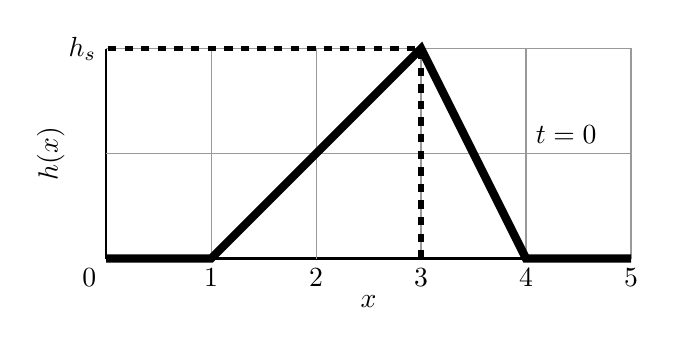
\begin{tikzpicture}[scale=4/3]
        \draw [thick] (0,0) -- (5,0);
        \draw [thick] (0,0) -- (0,2) node [midway, sloped, yshift=2em] {\(h(x)\)};
        \node [below left] at (0,0) {0};
        \node [left] at (0,2) {\(h_s\)};
        \foreach \x in {1,2,3,4,5} {
            \node [below] at (\x,0) {\x};
            \draw [black!40] (\x,0) |- (0,1);
            \draw [black!40] (\x,0) |- (0,2);
        }
        \draw [dashed,line width=2pt] (3,0) |- (0,2);
        \draw [line width=3pt] (0,0) -- (1,0) -- (3,2) -- (4,0) -- (5,0);
        \path (2,0) -- (3,0) node [midway, below, yshift=-1em] {\(x\)};
        \node [above right] at (4,1) {\(t=0\)};
    \end{tikzpicture}
\end{center}

\begin{enumerate}[label=(\alph*)]
    \item Como a função de onda tem o formato \(f(x+vt)\), com \(x\) em \si{cm}
        e \(t\) em \si{s}, temos que \(v= \SI{5}{cm/s}\)
    \item Como a função de onda tem o formato \(f(x+vt)\), temos que o sentido de
        propagação do pulso é negativo (\(-x\))
    \item O pulso se propaga para a \textit{esquerda} com velocidade de \SI{5}{cm/s}, 
        de forma que após \SI{2}{s} temos o mesmo gráfico mas com os valores do eixo \(x\)
        diminuídos em \(5*2=10\):

        \begin{center}
            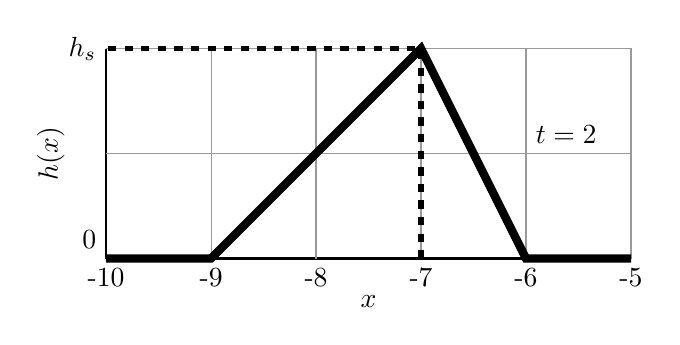
\begin{tikzpicture}[scale=4/3]
                \draw [thick] (-10,0) -- (-5,0);
                \draw [thick] (-10,0) -- (-10,2) node [midway, sloped, yshift=2em] {\(h(x)\)};
                \node [below] at (-10,0) {-10};
                \node [above left] at (-10,0) {0};

                \node [left] at (-10,2) {\(h_s\)};
                \foreach \x in {-9,-8,-7,-6,-5} {
                    \node [below] at (\x,0) {\x};
                    \draw [black!40] (\x,0) |- (-10,1);
                    \draw [black!40] (\x,0) |- (-10,2);
                }
                \draw [dashed,line width=2pt] (-7,0) |- (-10,2);
                \draw [line width=3pt] (-10,0) -- (-9,0) -- (-7,2) -- (-6,0) -- (-5,0);
                \path (-8,0) -- (-7,0) node [midway, below, yshift=-1em] {\(x\)};
                \node [above right] at (-6,1) {\(t=2\)};
            \end{tikzpicture}
        \end{center}

    \item Do gráfico vemos que em \(t=0\) vemos que \(h\) é igual a \(h_s=2\) em \(x=3\) e esse valor cai linearmente
        à medida que o pulso avança para a esquerda. Em \(t=0\) temos que \(h=0\) (valor mínimo de \(h\)) em \(x=4\) e para
        essa ''parte'' do pulso chegar em \(x=3\) vai demorar \((4-3)/5=\num{0.2}\). Com essas informações, temos que 

        \begin{center}
            \begin{tikzpicture}[scale=40/3]
                \draw [thick] (0,0) -- (0,0.2) node [midway, sloped, yshift=2em] {\(h(x)\)};
                \node [below left] at (0,0) {0};
                \node [left] at (0,0.2) {\(h_s\)};

                \draw [thick] (0,0) -- (0.4,0) node [right] {t};

                \draw (0,0.2) -- (0.2,0) node [below] {\num{0.2}};

                \node at (0.3,0.1) {\(x=3\)};
            \end{tikzpicture}
        \end{center}
\end{enumerate}

\subsection*{Questão 2}

A equação de uma onda transversal que se propaga em uma corda muito longa é 
\(y = \num{6.0} \sen(\num{0.020}\pi x + \num{4.0}\pi t)\), em que \(x\) e
\(y\) estão em centímetros e \(t\) em segundos. Determine (a) a amplitude,
(b) o comprimento de onda, (c) a frequência, (d) a velocidade, (e) o 
sentido de propagação da onda e (f) a máxima velocidade transversal de uma 
partícula da corda. (g) Qual é o deslocamento transversal em 
\( x = \SI{3.5}{cm}\) para \(t = \SI{0,26}{s}\)?

\textit{Solução}:

\begin{enumerate}[label=(\alph*)]
    \item Como \(-1 \leq \sen{\theta} \leq 1\), temos que a amplitude é igual a \SI{6.0}{cm}
    \item O coeficiente da variável \(x\) é \(k=\num{0.020}\pi\) e como \(\lambda = 2\pi/k = 2/\num{0.020}=\SI{100}{cm}\)
    \item O coeficiente da variável \(t\) é \(\omega = \num{4.0}\pi\) e como \(f=\omega/2\pi = \SI{2.0}{Hz}\)
    \item A velocidade é dada por \(v=\lambda f = 100 * 2 = \SI{200}{cm/s} \)
    \item O sinal do coeficiente da variável \(t\) é positivo, logo o sentido é negativo (\(-x\))
    \item A velocidade transversal (perpendicular à direção de propagação) é 
        \(\partial y/\partial t = \num{24\pi}\cos(\num{0.020}\pi x + \num{4.0}\pi t)\) e como
        \(-1 \leq \cos{\theta} \leq 1\), temos que a máxima velocidade transversal é \SI{24\pi}{cm/s}
    \item Basta substituir em \(y\) os valores de \(x\) e \(t\) dados, ou seja
        \(
        y = \num{6.0} \sen{(\num{0.020}\pi * \num{3.5} + \num{4.0}\pi * \num{0.26})} = \SI{-2.03}{cm}
        \)
\end{enumerate}

\subsection*{Questão 3}

Um pêndulo simples, com \SI{20}{cm} de comprimento e \SI{5.0}{g} de massa, está suspenso
em um carro de corrida que se move a uma velocidade constante de \SI{70}{m/s}, descrevendo
uma circunferência com \SI{50}{m} de raio. Se o pêndulo sofre pequenas oscilações na direção
radial em torno da posição de equilíbrio, qual é a frequência das oscilações?

\textit{Solução}:

\begin{itemize}
    \item Temos uma força resultante \(\vec{F_R} = -mg \hat{z}-mv^2/R \hat{r}\) que tem módulo
        \(F_R = m\sqrt{g^2 + v^4/R^2}\) e faz um ângulo \(\alpha = \arctg{(v^2/Rg)}\), \(0 \leq \alpha < \SI{90}{\degree}\),
        com o semieixo \(-z\)

        \begin{center}
            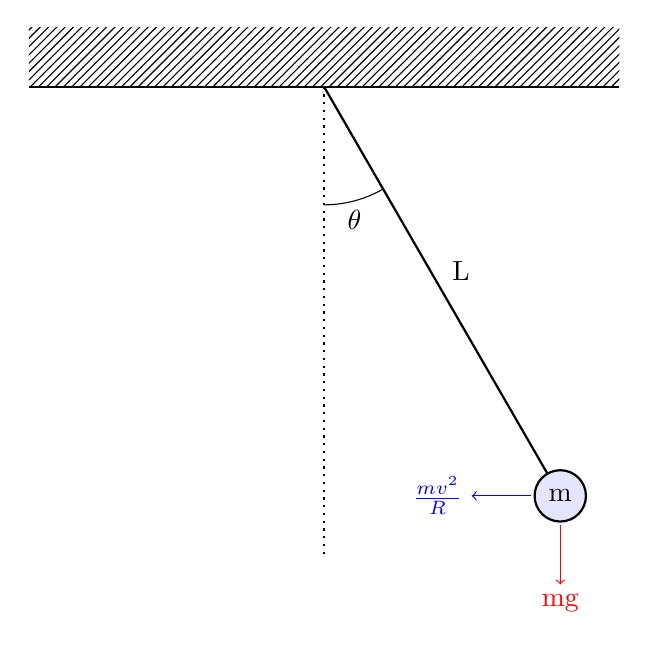
\begin{tikzpicture}[scale=3/4,
                ground/.style={fill,pattern=north east lines,draw=none,minimum width=0.3,minimum height=0.6}
                ]
                \draw [ground] (0,0) rectangle (10,1);
                \draw [thick] (0,0) -- (10,0);
                \draw [dotted,thick] (5,0) -- (5,-8);
                \draw [thick] (5,0) -- ++(-60:8) node [midway, above right] {L} node [circle, fill=blue!10, draw=black] {m} coordinate (A);
                \draw [red,->] (A) ++(0,-0.5) -- ++(0,-1) node [below] {mg} ;
                \draw [blue,->] (A) ++(-0.5,0) -- ++(-1,0) node [left] {\(\frac{mv^2}{R}\)} ;
                \draw (5,-2) arc (270:300:2) node [midway, below] {$\theta$};
            \end{tikzpicture}
        \end{center}

    \item Ou seja
        \[
            \tau = -Lm\sqrt{g^2+\frac{v^4}{R^2}}\sen{(\theta+\alpha)}
        \]
    \item Assim, com \(\tau = I\alpha=I d^2 \theta/dt^2\) e \(I=mL^2\), temos
        \[
            \frac{d^2 \theta}{dt^2}=-\frac{1}{L}\sqrt{g^2+\frac{v^4}{R^2}}\sen{(\theta+\alpha)}
        \]
    \item Quando \(\theta +\alpha \to 0\), temos \(\sen(\theta+\alpha) \to \theta + \alpha\), ou seja
        \[
            \frac{d^2 \theta}{dt^2}=-\frac{1}{L}\sqrt{g^2+\frac{v^4}{R^2}}(\theta+\alpha) \implies
            \frac{d^2 u}{dt^2}=-\omega^2 u
        \]
        onde
        \[
            \omega = \sqrt{\frac{\sqrt{g^2+\frac{v^4}{R^2}}}{L}}
        \]
        e \(u=\theta + \arctg({v^2/Rg})\)

    \item Finalmente\footnote{Como a questão não pede para demonstrar ou achar a fórmula para \(\omega\), pode-se apenas usá-la}, 
        temos que 
        \[
            f=\frac{\omega}{2\pi} = 
            \frac{1}{2\pi} \sqrt{\frac{\sqrt{\num{9.8}^2+\dfrac{\num{70}^4}{\num{50}^2}}}{\num{20e-2}}}
            = \SI{3.53}{Hz}
        \]
\end{itemize}
\end{document}
